%%%%%%%%%%%%%%%%%%%%%%%%%%%%%%%%%%%%%%%%%%%%%%%%%%%%%%%%%
%  PATT2 FORM VERSION 02/2003 - TEMPLATE                %
%%%%%%%%%%%%%%%%%%%%%%%%%%%%%%%%%%%%%%%%%%%%%%%%%%%%%%%%%
%  ENTER THE INFORMATION BETWEEN THE CURLY BRACKETS     %
%%%%%%%%%%%%%%%%%%%%%%%%%%%%%%%%%%%%%%%%%%%%%%%%%%%%%%%%%
%  DO NOT EDIT THE PATT2.STY FILE IN ANY WAY            %
%%%%%%%%%%%%%%%%%%%%%%%%%%%%%%%%%%%%%%%%%%%%%%%%%%%%%%%%%

%%%%%%%%%%%%%%%%%%%%%%%%%%%%%%%%%%%%%%%%%%%%%%%%%%%%%%%%%
% the default font size must not be altered from 11pt.  %
% proposals written in a smaller font will be rejected  %
%%%%%%%%%%%%%%%%%%%%%%%%%%%%%%%%%%%%%%%%%%%%%%%%%%%%%%%%%
                                                       
\documentclass[11pt]{article}
\usepackage{patt2}

% Allow epsfig, psfig or graphicx packages

\usepackage{epsfig}
\usepackage{psfig}
\usepackage{graphicx}

\usepackage{color}
\definecolor{ref}{rgb}{0,0,1}
\def\citecol{\color{ref}}
\usepackage{multicol}


% Uncomment below if using pdflatex
%\usepackage{epstopdf}
%\pdfpageheight=11.69in
%\pdfpagewidth=8.26in

\typeout{This is the PATT2 (Optical/IR) blank LaTeX form}

% add any personal macros here

% end macros

\begin{document}

\telescope{INT}    % AAT, UKST, WHT, INT or UKIRT
\semester {2023B}    % eg 2003B

\category {4}    % Scientific Category (enter a number):
                % 1 Solar system and extrasolar planets
                % 2 ISM, CSM, PNe, including star formation
                % 3 Stars and stellar populations (galactic and circum-galactic)
                % 4 Low-z universe
                % 5 High-z universe
 
\relatedapps {}{}{}{}{}{}{}{}{} % Coordinated PATT applications {x}
% in order  AAT,UKST,WHT,INT,UKIRT,JCMT,Gemini,LT,MERLIN

%%%%%%%%%%%%%%%%%%%%%%%%
% PAGE 1 OF PATT2 FORM %
%%%%%%%%%%%%%%%%%%%%%%%%

% PI information

\pisurname     {}                % Surname
\pititle       {}                % Mr/Mrs/Ms/Miss/Dr/Prof
\pifirstname   {}                % First name
\pistatus      {}                % Post held
\piaddressone  {}                % Name of Institute
\piaddresstwo  {}                % Postal Address
\piaddressthree{}                % Postal Address
\piphone       {}                % Phone number
\pifax         {}                % Fax number
\piemail       {}                % email address
\piobserver    {}                % Is the PI going to observe? {Yes/No}

% collaborator 1

\collabonename    {Tobias G\'eron}             % Name of first collaborator
\collaboneinst    {University of Oxford}             % Name of Institute
\collaboneobserver{Yes}             % Will collaborator observe? {Yes/No}

% collaborator 2

\collabtwoname    {Dr Rebecca Smethurst}
\collabtwoinst    {University of Oxford}
\collabtwoobserver{Yes}

% collaborator 3

\collabthreename    {Dr Brooke Simmons}
\collabthreeinst    {Lancaster University}
\collabthreeobserver{Yes}

% collaborator 4

\collabfourname    {Prof Chris Lintott}
\collabfourinst    {University of Oxford}
\collabfourobserver{Yes}

% note additional collaborators can be added by inserting multiple
%names into these entries.



% proposal information 

\title      {Are strong and weak bars different?}                % Brief title  (12 words only)

\abstract   {Recent theoretical and observational work constraining the influence of mergers on galaxy evolution and growth has focused attention on the secular processes which must shape the local galaxy population, including the presence of a bar. In galaxies with strong and dominant bars, the bar can either trigger starbursts or dynamically heat gas, preventing star formation, in either case triggering a quench. Yet such strongly barred galaxies represent a minority of the disk galaxy population. We use a newly assembled sample to determine for the first time the effect of even a weak bar feature on the galaxy, using spectra from IDS on the INT to measure gas inflow in samples of weakly barred, strongly barred and control systems. These observations represent an important step in understanding the contribution of barred morphological quenching to the bulk of the disk galaxy population.

% summary of proposed observations
% add your abstract here.  the font size must not be smaller 
% than the default in the style-file


}                


% Instrument requirements

\focalstation       {Cassegrain}        % eg prime,f/3.3,f/8,f/15,f/36,cs/36
\instrument         {IDS}        % eg RGO spec, UCLES, UHRF, Taurus, TTF, IRIS
                              % prime focus imager, LDSS etc
\detector           {EEV10}        % which chip do you want to use?
\gratingsandfilters {R300V}        % eg UBVRI,H$\alpha$,1200R,etc

\timerequested  {5}{}{}{Nights}      % No. of {Dark},{Grey},{Bright}, 
                              % {Weeks/Nights/Hours}
\minuseful      {5}{}{}        % Minimum number of useful {D},{G},{B} 
\lttotaltime    {}{}{}{}      % For long term proposals indicate the
                              % TOTAL requested {D},{G},{B},{W/N/H}


%%%%%%%%%%%%%%%%%%%%%%%%
% PAGE 2 OF PATT2 FORM %
%%%%%%%%%%%%%%%%%%%%%%%%

\prefdates            {(late) Sep, (early) Oct, Jan}      % Preferred dates, eg Jan,Feb
\impossdates          {Aug, Nov, Dec}      % Impossible dates, eg Mar,Apr
\datesjustification   {Targets have wrong RAs}      % Why impossible? eg wrong RAs, etc
\simultaneous         {}      % Simultaneous with other tels/satellites?
\othertimeconstraints {}      % eg Moon phase/position,specific dates
\serviceobservingyes  {}      % Observations to be done as Service? {x}
\serviceobservingno   {}      % or not {x}
\serviceobservingmaybe{}      % or maybe {x}
\supporteverynight    {}      % Support astronomer every night? {x}
\supportnone          {}      % No support astronomer? {x}
\supportfirstnight    {X}      % Support astronomer first night only? {x}
                              % (This is the only option for ING)

% target info                 % Target RA,Dec,Mags,Colours,Exp Time

\targetinfo{
    NB\_1 \qquad\qquad\qquad\quad 00 58 48.8506 \qquad\qquad\quad 00.587277 \qquad\qquad\quad 13.51 \qquad\qquad\quad 0.54 \qquad\qquad\qquad\qquad 11\\
    NB\_2 \qquad\qquad\qquad\quad 00 10 39.3502 \qquad\qquad\quad -0.052891 \qquad\qquad\quad 14.32 \qquad\qquad\quad 0.53 \qquad\qquad\qquad\qquad 12\\
    WB\_1 \qquad\qquad\qquad\quad 01 24 55.2247 \qquad\qquad\quad 00.211588 \qquad\qquad\quad 14.8 \qquad\qquad\quad 0.49 \qquad\qquad\qquad\qquad 64\\
    WB\_2 \qquad\qquad\qquad\quad 00 57 41.8827 \qquad\qquad\quad 15.06805 \qquad\qquad\quad 14.89 \qquad\qquad\quad 0.54 \qquad\qquad\qquad\qquad 110\\
    SB\_1 \qquad\qquad\qquad\quad 01 36 00.1502 \qquad\qquad\quad 00.663477 \qquad\qquad\quad 13.19 \qquad\qquad\quad 0.69 \qquad\qquad\qquad\qquad 19\\
    SB\_2 \qquad\qquad\qquad\quad 01 07 14.2381 \qquad\qquad\quad 13.955141 \qquad\qquad\quad 13.76 \qquad\qquad\quad 0.69 \qquad\qquad\qquad\qquad 52\\
    SB\_3 \qquad\qquad\qquad\quad 00 35 14.5384 \qquad\qquad\quad 00.695974 \qquad\qquad\quad 14.74 \qquad\qquad\quad 0.59 \qquad\qquad\qquad\qquad 65\\
    \rm{and} \rm{7} \rm{other} \rm{similar} \rm{targets}. Magnitudes are r-band magnitudes from the Legacy survey. Colour is the g-r colour obtained from Petrosian magnitudes from SDSS. Exposure time is in minutes.

%enter target information here.  this should include name, ra, dec
%and some indication of magnitude, line flux etc.  it is OK to use
%a small font here.

}

% LIST ALL SIMILAR/SUPPORTING APPLICATIONS TO ANY PATT OR OTHER TIME
% ASSIGNMENT COMMITTEE  
% You must include a brief description of any
% other applications whose targets or science goals are similar to 
% those requested here

\otherapplications{
\begin{tabular}[t]{p{1.6in}p{5.0in}}
%Telescope/Committee & Short title of programme  \\
\end{tabular}
}


%%%%%%%%%%%%%%%%%%%%%%%%%%%%%%%%%%%%%%%%%%%%%%%%%%%
% PAGE 3 OF PATT2 FORM - SCIENTIFIC JUSTIFICATION %
%%%%%%%%%%%%%%%%%%%%%%%%%%%%%%%%%%%%%%%%%%%%%%%%%%%

\sciencecase{
    Understanding the role that internal processes play in galaxy evolution is a key goal of modern astrophysics. An increasing body of evidence shows that galaxy evolution and growth is mainly driven by secular, or non-merger driven, processes ; {\citecol Kaviraj et al. (2012)}$^{[1]}$, for example, have shown that only 27\% of star formation is triggered by major or minor mergers. Recent work in cosmological simulations (e.g. {\citecol Martin et al. 2018}$^{[2]}$, {\citecol McAlpine et al. 2020}$^{[3]}$), following observational work by {\citecol Simmons, Smethurst \& Lintott (2017)}$^{[4]}$, also reveals the importance of secular processes.

    It is therefore important to identify the dominant mechanisms responsible for galaxy growth and the quenching (or cessation) of star formation. One candidate process is the funneling of gas from the outskirts of a galaxy by a galactic-scale bar ({\citecol Athanassoula 1992}$^{[5]}$); bars are thought to remove gas needed for star formation in the outer regions and deposit it in the centre, where it either triggers a starburst or is too dynamically hot to be used for future star formation ({\citecol Zurita et al. 2004}$^{[6]}$, {\citecol Sheth et al. 2005}$^{[7]}$, {\citecol Jogee et al. 2005}$^{[8]}$), in either case causing a quench.% (see Figure 2). 
    
    However, this process has only been observed in galaxies with strong bars, where the bar is the dominant feature. Most previous studies have focussed their efforts on the strong bar population ({\citecol Rosas-Guevara et al. 2020}$^{[9]}$, {\citecol Newnham et al. 2020}$^{[10]}$, {\citecol Khoperskov et al. 2018}$^{[11]}$) which are easier to detect since they are brighter and constitute the main feature of the galaxy. Yet a large range of bar strengths are seen across the galaxy population with a broad distribution of bar lengths, widths and relative sizes, and systems with strong bars are in the minority ({\citecol Masters et al. 2011}$^{[12]}$). While strong bars appear more frequently in quiescent galaxies - an indication that the presence of the bar may be effective in quenching - galaxies with weaker bars are evenly distributed between star forming and quiescent galaxies. \textbf{This suggests that weak and strong bars may not affect a galaxy in the same way} ({\citecol G\'eron et al. 2021}$^{[13]}$). The absence - until now - of a large sample of weak bars has prevented equivalent observations for weakly barred systems.
    %; or don't make the distinction between weak and strong bars ({\citecol Cheung et al. 2013}$^{[13AA]}$, {\citecol Masters et al. 2011}$^{[12]}$)

    %{\citecol Cuomo et al. 2019}$^{[14AA]}$ measured the bar pattern speed in a small sample of 16 weakly barred spirals, finding no significant differences between strongly and weakly barred systems, which suggests that any differences must be due to the way the bar interacts with the gas. 
    
    In this project we propose to observe a sample (see Figure 1) of strong and weak bars along with a control sample of unbarred galaxies. These galaxies are selected from a new Galaxy Zoo sample, called Galaxy Zoo DESI, which distinguishes between strong and weak bars ({\citecol Walmsley et al. 2023}$^{[14]}$). We propose to use the IDS spectrograph on the INT to obtain spectra parallel and perpendicular to the bar (and, time permitting, halfway in between for each target). The flexibility provided by the choice of gratings makes IDS the ideal instrument to achieve our science goals. %Whilst these galaxies would be interesting targets for an IFU survey, no such survey has yet included a sufficiently large number of these systems for the study we propose here. Instead, observations with IDS will allow us to target a mass-matched sample of strong and weak bars across the star formation rate - stellar mass diagram and supplement the existing small number samples from IFU surveys such as MaNGA ({\citecol Bundy et al. 2015}$^{[17]}$). 
    
    The results of {\citecol G\'eron et al. 2023}$^{[15]}$ show that strong and weak bars have significantly different pattern speeds, which hints that there are differences in the gas kinematics of strong and weak bars as well. Resolving the emission lines in each target across a large range of wavelengths with IDS will allow us to determine the gas kinematics along and perpendicular to the bar. We will test whether there is a significant inflow of gas along both strong and weak bars, comparing the measurements to those taken outside the bar (and compared to the control sample of unbarred galaxies). We aim to definitely answer the question; do weak bars drive gas to the centre of a galaxy at the same or different rates to strong bars, and are they therefore capable of quenching? 

    Choosing a grating on the IDS which balances the spectral resolution while  targetting a large wavelength range will also allow us to determine the star formation rates within and outside strong and weak bars using $H\alpha$, $D_{\rm n}4000\rm$ and \textsc{[OIII]} ({\citecol Spindler et al. 2018}$^{[16]}$). These resolved star formation rates will be crucial to determining whether both weak and strong bars are responsible for any decrease in the star formation rate in these galaxies. This will allow us to determine if strong and weak bars are separate phenomenon. 

    We submitted a similar proposal for the 2022B semester and we were awarded 5 dark nights. Unfortunately, due to storm Hermine, we were only able to observe one strongly barred target. Nevertheless, for this one target, we found interesting differences in the amount of $H\alpha$ between the parallel and perpendicular slit, with significantly more $H\alpha$ flux found in the parallel slit, as shown in Figure 2. This proof-of-concept shows the viability of this study and indicates that it is worthwhile to observe the entire sample.
    
    We will publish two papers as a result of these observations: (1) measuring the gas kinematics to determine whether their bars allow gas to flow towards their centres and (2) constraining the star formation rates inside and outside of the bar to determine whether either strong or weak bars are directly responsible for quenching galaxies. With this work we aim to characterise the differing or similar effects of weak and strong bars to determine their overall contribution to galaxy evolution.  

% add your science case here.  

% proposals written in a font smaller than 11pt will be rejected


}

%%%%%%%%%%%%%%%%%%%%%%%%%%%%%%%%%%%%%%%%%%%%%%%%%%%%%%%%
% PAGE 3a OF PATT2 FORM - SCIENTIFIC JUSTIFICATION     %
% FOR PROPOSALS TO AAT, WHT or UKIRT FOR 8 OR MORE     % 
% NIGHTS, AND FOR  ALL (I.E. INCLUDING INT AND UKST)   %
% LONG-TERM AND COORDINATED PROPOSALS (INCLUDING THOSE %
% COORDINATED WITH NON-PATT TELESCOPES)                %
%%%%%%%%%%%%%%%%%%%%%%%%%%%%%%%%%%%%%%%%%%%%%%%%%%%%%%%%

\extendedsciencecase{

% continue your science case here ONLY if applying for 8 or 
% more nights to the AAT, WHT OR UKIRT, or if your proposal 
% is a long-term (multi-semester) proposal to the AAT, UKST, 
% WHT, INT or UKIRT, or if your proposal (to AAT, UKST, WHT, 
% INT or UKIRT) is coordinated with other telescopes (including 
% non-PATT telescopes).  

% Remember to comment IN the \makepatttwopagethreea command later 
% in this file if you have written an extended science case  

% proposals written in a font smaller than 11pt will be rejected

}


%%%%%%%%%%%%%%%%%%%%%%%%%%%%%%%%%%%%%%%%%%%%%%%%%%%%%%%%%%%%%%%%%%%%%%%%%%%%
% PAGE 4 OF PATT2 FORM - TECHNICAL INFORMATION (I) - FEASIBILITY, S/N, ETC %
%%%%%%%%%%%%%%%%%%%%%%%%%%%%%%%%%%%%%%%%%%%%%%%%%%%%%%%%%%%%%%%%%%%%%%%%%%%%


%%%%%% Line calculations
    % Halpha is at 6564.6 A
    % Hbeta is at 4862.7 A
    % OIII is at 4960.3 A  - 5008.2 A
    % Dn4000 is at 4000 A
    %
    % At our redshift range (0.01 - 0.05), this corresponds to:

    % 1+z = l_obs / l_emit => l_obs = (1+z) * l_emit
    % Halpha: 6630.2 - 6958.5 A
    % Hbeta: 4911.3 - 5154.5 A
    % OIII: 5009.9/5058.3 - 5257.9/5308.7 A
    % Dn4000: 4040 - 4200 A
    %
    % So (observed) line range is: 4911.3 - 6958.5 A
    %
    % Source: https://classic.sdss.org/dr3/products/spectra/vacwavelength.html


    %%%%%%% Resolution calculations
    % The (observed) line range is (exactly for our targets, not including Dn4000): 4929 - 6917 A.   
    % The dispersion for R300V grating on EEV10 is 1.87 A/pix.
    %
    % For minimum line range: 4929
    % ((4929 + 1.87) - 4929)/4929 * c[km/s] = 113.74 km/s
    %
    % For maximum line range: 6917
    % ((6917 + 1.87) - 6917)/6917 * c[km/s] = 81.05 km/s
    %
    % The spectral resolution is 81.05- 113.74 km/s
    %
    % Source: http://www.ing.iac.es/Astronomy/instruments/ids/idsgrat_tables.html

    %The MaNGA resolution is ~2000, whereas the R300V resolution is 1203.
    
    

    %Downtime found here: http://www.ing.iac.es/astronomy/observing/conditions/
    %Total observing time calculator: http://catserver.ing.iac.es/service/TTE.php




\technicalpage{

    The parent sample from which our galaxies are drawn is made up of galaxies with reliable bar classifications from GZ DESI ({\citecol Walmsley et al. 2023}$^{[14]}$). We volume limit our sample with a redshift range, $0.01 < z < 0.05$ and a magnitude limit $M_r < -18.96$. From our parent sample, we matched 7 galaxies with strong bars, 7 with weak bars and 7 without bars, for a total of 21 galaxies. This sample size and setup allows for a meaningful study of all bar types and will help us to disentangle any potential differences between weak and strong bars. In case of bad weather we would focus our efforts on the brightest targets and reduce the number of slit angles, which will allow us to still gain valuable insight into the effect of the bar on the gas kinematics.
    
    We chose targets which were not in the MaNGA target list ({\citecol Bundy et al. 2015}$^{[17]}$), CALIFA ({\citecol S\'anchez et al. 2012}$^{[18]}$) or SAMI ({\citecol Scott et al. 2005}$^{[19]}$), to avoid unnecessary duplicate observations. %Such broad IFU studies typically aim to observe a general sample of the galaxy population and thus have too few galaxies in that fit our specific requirements: three samples (strongly, weakly and unbarred galaxies) that are matched in mass, redshift and global SFR and that overlap with GZ DESI and ALFALFA (see below).
    \\
    The IDS spectrograph on the INT is ideal for observing this sample due to the flexibility of the gratings available. This allows us to optimise the wavelength range targeted against the spectral resolution in order to maximise the science output. We therefore propose to target the $H\alpha$ emission line in each of our sources with the R300V grating on the EEV10 detector, which still has a large enough wavelength range to also capture the $D_n4000\rm{\AA}$ break-$H\beta$-\textsc{[OIII]} region ($5067 < \textsc{[OIII]} \lambda_{emit} $[\rm{\AA}]$ < 5245$) with high efficiency. Targeting these regions of the spectrum specifically will allow us to observe a maximum number of emission lines with high resolution to derive precise gas kinematics whilst also allowing for an accurate determination of the resolved star formation rate in and outside the bar ({\citecol Spindler et al. 2018}$^{[16]}$). 

    The R300V grating has a dispersion of 1.87 \AA/pix. For the wavelength range we are interested in ($\sim$4929 - 6917 \AA), this translates to a resolution of $\sim$81 - 114 km/s. From the experience of the authors, the centroid of an emission line can be detected to $\sim$1/10th of a pixel. Given the dispersion of the R300V grating and a targetted SNR of $\sim$10, we expect to be able to characterise the uncertainty on the gas velocities up to $\sim$8 - 11 km/s. Simulations have shown that gas inflows due to bars can reach velocities of the order of $\sim$100 km/s ({\citecol Athanassoula, E. 1992}$^{[5]}$, {\citecol Kim et al. 2012}$^{[20]}$), which suggests that we will be able to detect them, or at the very least constrain their upper limits. We have also confirmed that all our targets have been detected by the ALFALFA Extragalactic HI Source Catalog ({\citecol Giovanelli et al. 2005}$^{[21]}$, {\citecol Haynes et al. 2018}$^{[22]}$) in order to ensure presence of HI gas. %{\citecol Athanassoula, E. 1994}$^{[X]}$, %Moreover, studies on the gas kinematics of galaxies have been done before with Mapping Nearby Galaxies at Apache Point Observatory (MaNGA) on the the Sloan 2.5 m telescope, which has a resolving power of $\sim$2000 and an instrumental dispersion of $\sim70$ km/s ({\citecol Bundy et al. 2015}$^{[X]}$, {\citecol Westfall et al. 2019}$^{[X]}$). The similar sized telescope and instrumental dispersion gives us more confidence that we will be able to observe gas kinematics, even though the resolution of the R300V is slightly lower (1203 at 4500\AA). 

    We want to measure the gas flow along and perpendicular to the bar and compare it for weak and strong bars. In order to do this, we propose to align the slit parallel and perpendicular to the bar (unbarred galaxies will have the slit aligned along the major and minor axes). Additionally, time permitting, to more easily isolate non-axisymmetric motion, we are planning to align the slit 45$^{\circ}$ away from the bar (or major axis for unbarred galaxies) as well. In order to derive an accurate measure of the gas inflow rates in our targets, we need to be able to determine the gas kinematics. We will utilise the tried and tested penalized pixel-fitting method (\textsc{PPXF}) spectral fitting code ({\citecol Cappellari \& Emsellem 2004}$^{[23]}$) to derive the velocity of the gas along the bar for each of our targets. To do this we require a high signal-to-noise ratio (SNR) to ensure that each of the emission lines in the sample are well resolved. We've used the Exposure Time Calculator SIGNAL using surface brightness measurements based on DESI r-band magnitudes to calculate appropriate exposure times to achieve a SNR of 10. However, we note that our science goals will still be possible if observations are limited to lower SNR (e.g. SNR $>$ 3) due to seeing limitations or time constrains. While using the ETC, we've assumed negligible sky background on dark sky nights with respect to the read noise and taken into account the quantum efficiency of the detector at the redshifted wavelength of $H\alpha$ ($6641 < \lambda_{emit} $[\rm{\AA}]$ < 6874$). Given these requirements the total on source time is 26.5 hours, assuming a seeing of 1" and optimal airmass conditions. The minimum (maximum) exposure time for a single source is $\sim$ 12 (145) minutes. 
    
    Using this information combined with the overhead estimates from the IDS Total Observing Time Estimator, we calculate that we can observe all 21 targets in 4.3 (rounded up to 5) nights of dark skies in October 2023 of the 2023B semester.  %Downtime is 34% for January %and assuming an average weather downtime of 25\% in September

    We also applied for and were awarded four nights of observing time for this project during the 2020B, 2021B and 2022B semesters, but due to extreme weather conditions and the volcano erupting we were not able to observe much in any semester.

    Finally, we want to note that the targets presented here are valid if we receive time in September/October. We can also construct a similar sample in case we receive telescope time in January.

% add any technical details you wish to transmit to the panel and
% technical assessor here. you may also include references here
% as well as on the next page

% proposals written in a font smaller than 11pt will be rejected


}

%%%%%%%%%%%%%%%%%%%%%%%%%%%%%%%%%%%%%%%%%%%%%%%%%%%%%%%%%%%%%%%%%%%%%%%%%%%%%%
% PAGE 4a OF PATT2 FORM - TECHNICAL INFORMATION (II) - REFERENCES, FIGS, ETC %
%%%%%%%%%%%%%%%%%%%%%%%%%%%%%%%%%%%%%%%%%%%%%%%%%%%%%%%%%%%%%%%%%%%%%%%%%%%%%%

\figsandrefspage{

    \begin{flushleft}
        \begin{multicols}{2}
        $[1]$ Kaviraj et al. 2013, MNRAS, 429, L40
        \\
        $[2]$ Martin et al. 2018, MNRAS, 476, 2801
        \\	
        $[3]$ McAlpine et al. 2020, MNRAS, 494, 5713
        %https://ui.adsabs.harvard.edu/abs/2020MNRAS.494.5713M/abstract
        \\
        $[4]$ Simmons, Smethurst \& Lintott, 2017, MNRAS, 470, 1559
        \\	
        %$[3]$ Cappellari \& Emsellem, 2004, PASP, 116, 138	
        %\\
        %$[4]$ Hoyle et al. 2011, MNRAS, 415, 4	
        %\\
        $[5]$ Athanassoula 1992, MNRAS, 259, 345 %https://ui.adsabs.harvard.edu/abs/1992MNRAS.259..345A/abstract
        \\
        $[6]$ Zurita et al. 2004, A\&A, 413 %https://ui.adsabs.harvard.edu/abs/2004A%26A...413...73Z/abstract
        \\
        $[7]$ Sheth et al. 2005, ApJ, 632, 1 
        %https://ui.adsabs.harvard.edu/abs/2005ApJ...632..217S/abstract
        \\
        $[8]$ Jogee et al. 2005, ApJ, 630, 2 
        %https://ui.adsabs.harvard.edu/abs/2005ApJ...630..837J/abstract
        \\
        $[9]$ Rosas-Guevara et al. 2020, MNRAS, 491, 2547
        %https://ui.adsabs.harvard.edu/abs/2020MNRAS.491.2547R/abstract
        \\
        $[10]$ Newnham et al. 2020, MNRAS, 492, 4697
        %https://ui.adsabs.harvard.edu/abs/2020MNRAS.492.4697N/abstract
        \\
        $[11]$ Khoperskov et al. 2018 A\&A 609, A60
        %https://ui.adsabs.harvard.edu/abs/2018A%26A...609A..60K/abstract
        \\
        %$[13AA]$ Cheung et al. 2013, ApJ 779, 2
        %https://ui.adsabs.harvard.edu/abs/2013ApJ...779..162C/abstract
        %\\
        %$[14AA]$ Cuomo et al. 2019, A\&A, 632, A51
        %https://ui.adsabs.harvard.edu/abs/2019A%26A...632A..51C/abstract
        %\\
        $[12]$ Masters et al. 2011, MNRAS 411, 2026
        %https://ui.adsabs.harvard.edu/abs/2011MNRAS.411.2026M/abstract
        \\
        $[13]$ G\'eron et al. 2021, MNRAS, 507, 4389
        %https://ui.adsabs.harvard.edu/abs/2021MNRAS.507.4389G/abstract
        \\
        $[14]$ Walmsley et al. 2023, in preparation
        \\
        $[15]$ G\'eron et al. 2023, accepted for publication in MNRAS
        %https://ui.adsabs.harvard.edu/abs/2023arXiv230205464G/abstract
        \\
        $[16]$ Spindler et al. 2018, MNRAS, 476, 580
        %https://ui.adsabs.harvard.edu/abs/2018MNRAS.476..580S/abstract
        \\
        $[17]$ Bundy et al. 2015, ApJ, 798, 7
        \\
        %$[17AA]$ Willett et al. 2013, MNRAS, 435, 1179
        %https://ui.adsabs.harvard.edu/abs/2008MNRAS.389.1179L/abstract
        %\\
        $[18]$ S\'anchez et al. 2012, A\&A 538, A8
        \\
        $[19]$ Scott et al. 2005, MNRAS, 481, 2
        %https://ui.adsabs.harvard.edu/abs/2018MNRAS.481.2299S/abstract
        \\
        $[20]$ Kim et al. 2021, ApJ, 747, 1
        %https://ui.adsabs.harvard.edu/abs/2012ApJ...747...60K/abstract
        \\
        $[21]$ Giovanelli et al. 2005, AJ 130, 6
        %https://ui.adsabs.harvard.edu/abs/2005AJ....130.2598G/abstract
        \\
        $[22]$ Haynes et al. 2018, ApJ, 861, 1
        %https://ui.adsabs.harvard.edu/abs/2018ApJ...861...49H/abstract
        \\
        $[23]$ Cappellari \& Emsellem, 2004, PASP, 116, 138
        

        \end{multicols}
        
        \end{flushleft}
    
    
        \centering{
        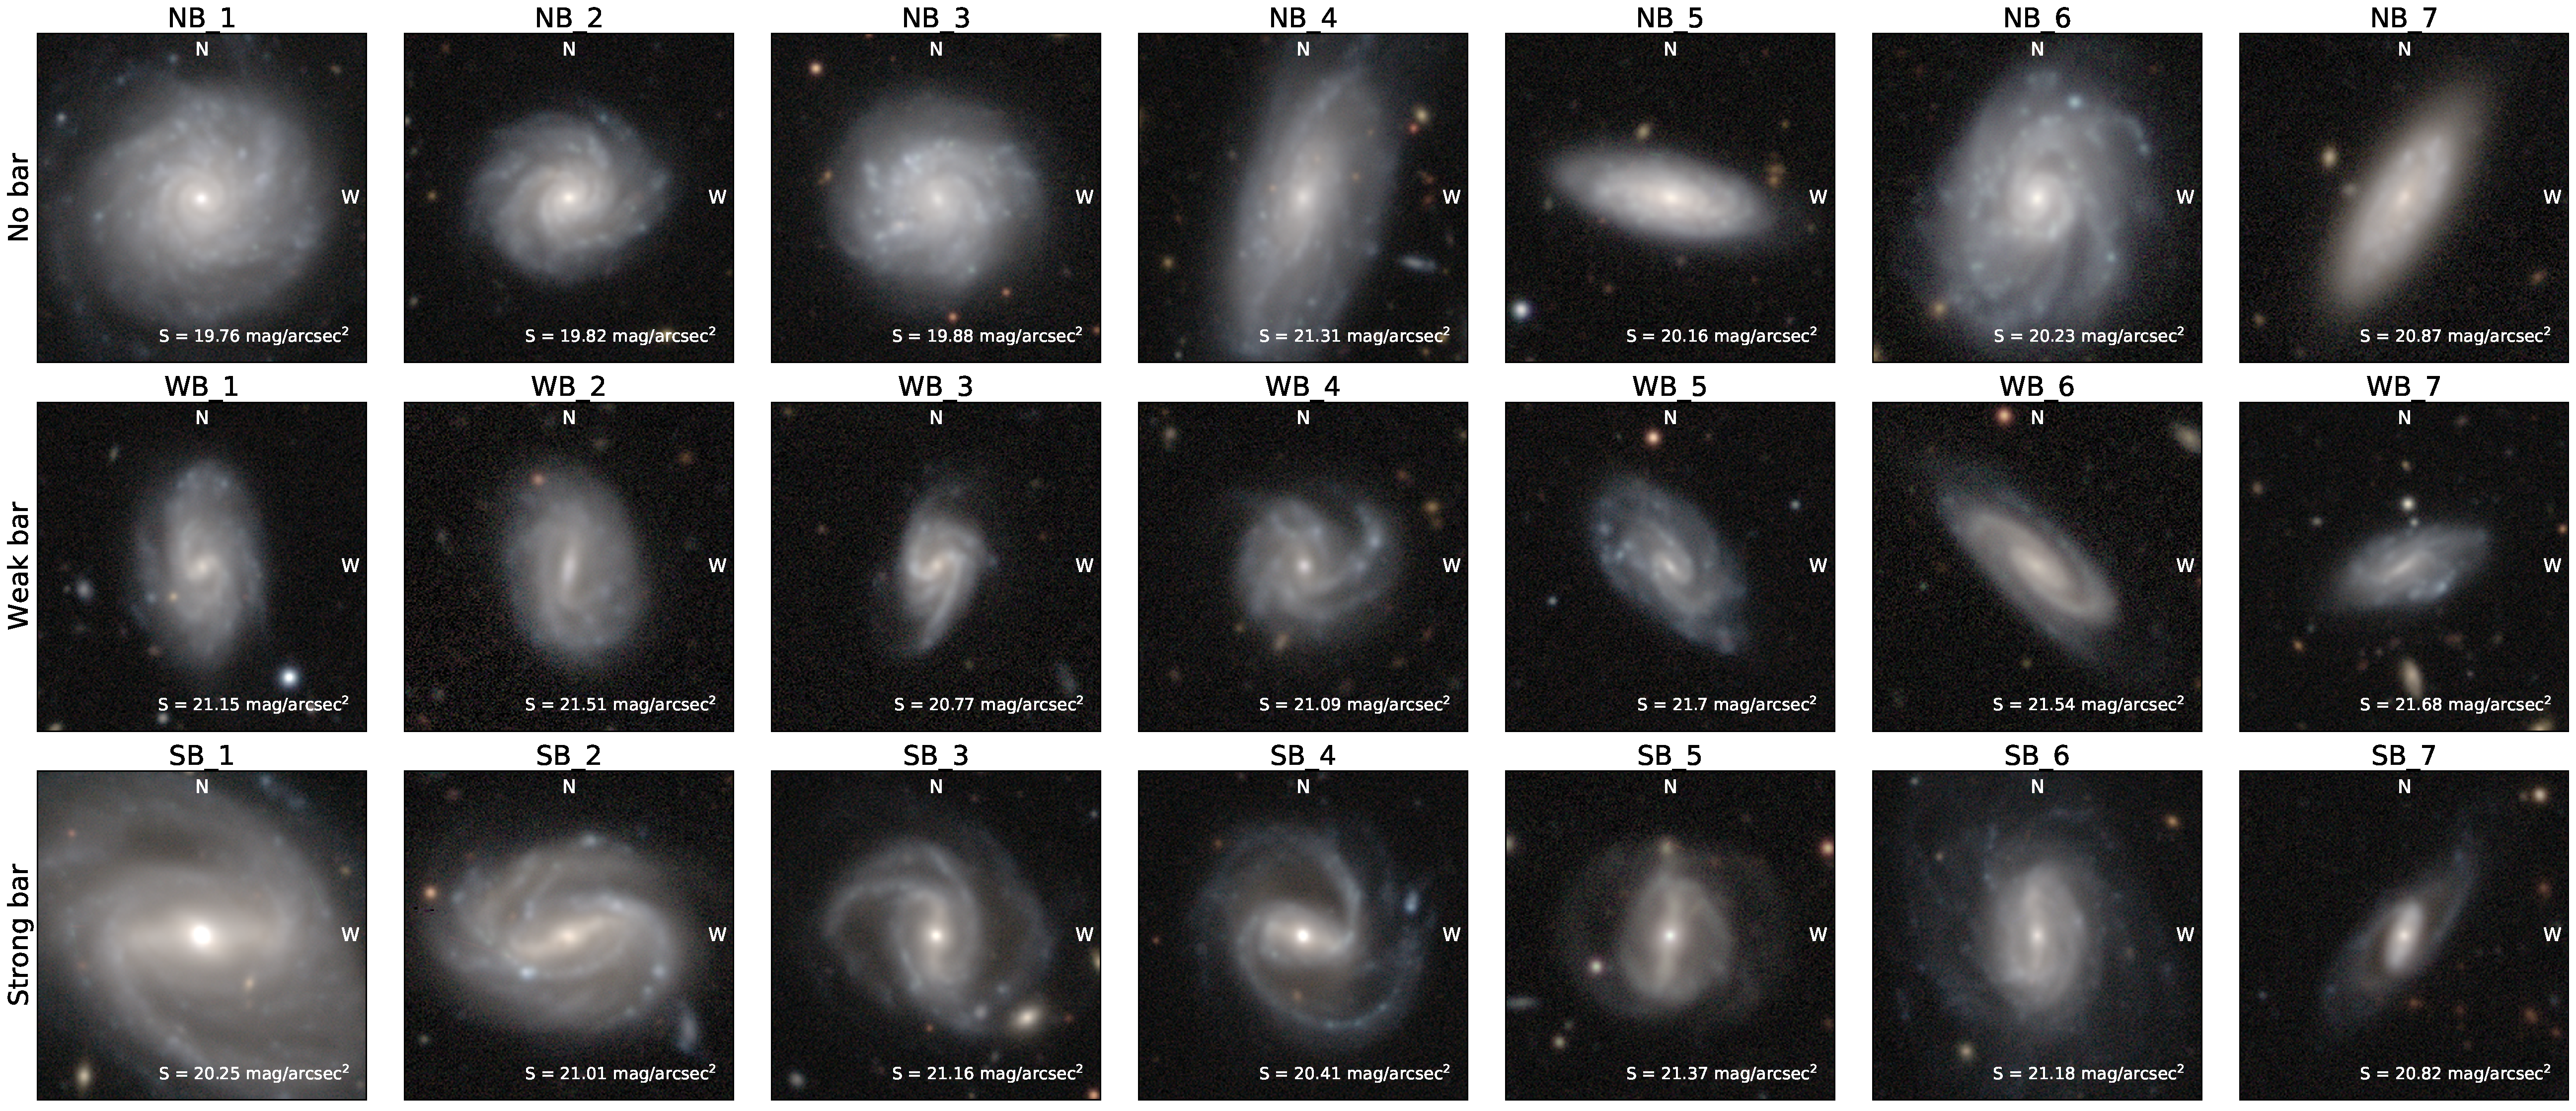
\includegraphics[width=0.7\textwidth]{targets_final.pdf}}
        \\
        \begin{flushleft}
        \small{Figure 1: Mosaic of postage stamps obtained from the DESI Legacy survey of targets in this sample ($0.01 < z < 0.05$). The sample is split into no bars (top; our control sample), weak bars (middle) and strong bars (bottom), which are mass-matched along each column. The surface brightness of each source is also noted. Each image is 64 arcseconds across.}
        \end{flushleft}


        \centering{
        \includegraphics[width=0.6\textwidth]{SB5_spectra.png}}
        \\
        \begin{flushleft}
        \small{Figure 2: The spectra of the one target (SB\_5) that was observed during the 2022B semester. The spectra with the slit placed parallel to the bar is shown in the top panel, while the spectra obtained with the slit placed perpendicular to the bar is shown in the bottom panel. The dashed vertical lines represent where it is expected to see $H\alpha$ emission.}
        \end{flushleft}

% add any figures, references etc here.  remember to embed your figures.


% proposals written in a font smaller than 11pt will be rejected

}

%%%%%%%%%%%%%%%%%%%%%%%%
% PAGE 5 OF PATT2 FORM %
%%%%%%%%%%%%%%%%%%%%%%%%

\backupprogram{In the case of poor seeing we will limit the number of sources targeted, decrease the number is slit angles and increase exposure times in order to still achieve optimal signal-to-noise ratios for a selection of our targets (initially those with shorter calculated exposure times). This will still allow the kinematics and star formation rates to be determined, but in a reduced sample size.}             % Summary of backup programme

\previous{                   % Previous applications (last 4 Sems)
\begin{tabular}[t]{p{1.5in}p{0.7in}p{0.8in}p{3.2in}}
%Patt No. & Award & clear nights & comments \\
I/2020B/09 & 4 nights & 0 clear nights & We could not observe any of our targets due to extremely bad weather caused by storm Filomena.\\
I/2021B/04 & 5 nights & 0 clear nights & We could not observe any of our targets to due the volcanic eruption on the island.\\
I/2022B/8 & 5 nights & 0.5 clear night & We could only observe one of our targets due to the extremely bad weather caused by storm Hermine.

\end{tabular}
}

\publications     {}         % List pubs with data from patt time (last 4 Sems)

\experience       {CL, BS, RS, TG and the PI have had experience observing with IDS on the INT. RS and BS have experience on the Shane 3-m at the Lick Observatory with both spectra and imaging. CL and RS have experience on the CSO, Mauna Kea (BS has remote experience of this telescope).}         % Experience of observers on other telescopes
\graduatestudent  {}{}       % Research student {Name of student}{Project}
\grant            {}{}{}     % {Name of PI}{Grant title}{Grant No.}
\nonstandardtravel{}         % Justify T&S for more than one UK observer
\otherexpenditure {}         % eg for freight etc.


%%%%%%%%%%%%%%%%%%%%%%%%%%%%%%%%%%%%%%%%%%%%%%%%%%%%%%%%%%%%%%%%%%%%%%%%%%%%%
% PAGE 6 OF PATT2 FORM - THIS SECTION IS REMOVED BY THE AAT DURING PROCESSING
% IF INCLUDED.  ING APPLICANTS SHOULD NOT ENTER ANYTHING HERE.
%%%%%%%%%%%%%%%%%%%%%%%%%%%%%%%%%%%%%%%%%%%%%%%%%%%%%%%%%%%%%%%%%%%%%%%%%%%%%

\shorttitle {}               % Ignore if you are an ING applicant.



\makepatttwopageone
\makepatttwopagetwo
\makepatttwopagethree

%%%%%%%%%%%%%%%%%%%%%%%%%%%%%%%%%%%%%%%%%%%%%%%%%%%%%%%%%%%%%%%%%%%%%
% COMMENT THE FOLLOWING LINE IN *ONLY* IF                           % 
%                                                                   %
% YOU ARE APPLYING FOR 8 OR MORE NIGHTS ON THE AAT, WHT OR UKIRT, OR% 
% YOUR PROPOSAL IS LONG-TERM FOR THE AAT, WHT, UKIRT OR INT, OR     % 
% YOUR PROPOSAL IS COORDINATED WITH OTHER TELESCOPES                % 
%                                                                   % 
% *AND* YOU HAVE USED THE CONTINUATION PAGE FOR YOUR SCIENTIFIC CASE% 
%%%%%%%%%%%%%%%%%%%%%%%%%%%%%%%%%%%%%%%%%%%%%%%%%%%%%%%%%%%%%%%%%%%%%
 
\makepatttwopagethreea

\makepatttwopagefour
\makepatttwopagefoura
\makepatttwopagefive

% FOR ING APPLICATIONS LEAVE THE FOLLOWING LINE COMMENTED OUT

%\makepatttwopagesix         

% FOR AAT APPLICATIONS YOU MAY LEAVE IT IN IF YOU WISH.  IT WILL NOT
% BE TRANSMITTED TO THE TAG HOWEVER.

\end{document}
